\documentclass[preprint,12pt]{elsarticle}

\usepackage{microtype}
\usepackage{amsmath,amssymb,amsthm,mathtools}
\usepackage{booktabs,tabularx,array,multirow}
\usepackage{graphicx}
\usepackage{caption}
\usepackage{subcaption}
\usepackage{placeins}
\usepackage{float}
\usepackage{xcolor}
\usepackage{enumitem}
\usepackage[hidelinks]{hyperref}
\usepackage{xurl}
\usepackage{seqsplit}
\biboptions{numbers,sort&compress}

\definecolor{navy}{HTML}{17365D}
\definecolor{teal}{HTML}{00897B}
\definecolor{orange}{HTML}{E76F51}
\hypersetup{
  colorlinks=true,
  breaklinks=true,
  linkcolor=navy,
  citecolor=teal,
  urlcolor=navy,
  pdftitle={Prefix-Causal Harm-Budget Projection for Cross-Domain Lithium-Ion Battery Capacity-Retention Estimation},
  pdfauthor={Yuyang Wu and Aiping Jiang}
}
\graphicspath{{figures/}}
\captionsetup{font=small,labelfont=bf,labelsep=period,justification=justified,singlelinecheck=false}
\setlist{nosep,leftmargin=1.5em}
\setlength{\emergencystretch}{3em}
\setlength{\textfloatsep}{14pt plus 2pt minus 4pt}
\setlength{\floatsep}{12pt plus 2pt minus 3pt}
\setlength{\intextsep}{12pt plus 2pt minus 3pt}
\setcounter{topnumber}{4}
\setcounter{bottomnumber}{2}
\setcounter{totalnumber}{5}
\renewcommand{\topfraction}{0.90}
\renewcommand{\bottomfraction}{0.80}
\renewcommand{\textfraction}{0.08}
\renewcommand{\floatpagefraction}{0.80}
\clubpenalty=10000
\widowpenalty=10000
\displaywidowpenalty=10000
\raggedbottom
\frenchspacing

\newtheorem{lemma}{Lemma}
\newtheorem{theorem}{Theorem}
\newtheorem{corollary}{Corollary}
\newcommand{\R}{\mathbb{R}}

\journal{Applied Energy}

\begin{document}
\begin{frontmatter}

\title{Prefix-Causal Harm-Budget Projection for Cross-Domain Lithium-Ion Battery Capacity-Retention Estimation}

\author[shu]{Yuyang Wu\fnref{orcid}}
\ead{1946929704@shu.edu.cn}
\ead{xiansuqiushui@gmail.com}
\author[shu]{Aiping Jiang\corref{cor1}}
\cortext[cor1]{Corresponding author}
\ead{ap724@shu.edu.cn}
\fntext[orcid]{ORCID: \href{https://orcid.org/0009-0002-4641-0753}{0009-0002-4641-0753}}
\address[shu]{SILC Business School, Shanghai University, 20 Chengzhong Road, Jiading District, Shanghai 201899, China}

\begin{abstract}
Fleet operators often update battery-health records from partial charge traces before reference-capacity tests are available. Cross-domain estimators adapt to new populations, but label-free deployment still lacks a joint contract that bounds each update's harm and prevents future data from rewriting issued estimates. We propose prefix-causal harm-budget projection (PCHP), which separates a protected source prediction from a candidate using changes since commissioning, then projects the candidate into a recursively feasible, non-increasing interval. Without distributional assumptions, PCHP bounds the per-record increase in absolute loss relative to the protected state by a declared budget for every hidden outcome and preserves every emitted prefix. Across $12$ development domains, $586$ cells, and $601{,}932$ records, PCHP reduced domain-equal mean absolute error (MAE) from $0.07524$ to $0.07038$; the paired change was $-0.00486$ ($95\%$ interval $[-0.00671,-0.00301]$), and $11/12$ domains improved. Protocol-frozen confirmation on six additional datasets with $659$ cells and $9{,}712$ records gave a PCHP-minus-development-selected-constant-offset MAE difference of $-0.00690$ ($95\%$ interval $[-0.01192,-0.00212]$), with gains on $5/6$ datasets and passage of all deterministic checks. An outcome-blind $45$-cell BaSyTec evaluation further confirmed transfer of the deployment constraint while exposing its accuracy trade-off. At a $5{:}1$ missed-degradation-to-unnecessary-review cost ratio, PCHP reduced continuous asymmetric cost by $7.54\%$, while the $0.01$ budget left the binary $80\%$ review decision unchanged. PCHP therefore enables adaptive cross-domain battery-health updates before outcomes arrive, with explicit control of predictive harm and operational trade-offs.
\end{abstract}

\begin{keyword}
lithium-ion battery \sep capacity retention \sep state of health \sep domain adaptation \sep online prediction \sep risk control \sep battery management
\end{keyword}

\end{frontmatter}

\section{Introduction}

Consider a battery-swapping operator introducing cells from a new supplier. At each service checkpoint, the operator must decide whether to continue routine operation or schedule a full diagnostic and maintenance review. Partial charging records are already available, but an accurate reference-capacity label is not: obtaining it requires a controlled characterization that interrupts normal service. Conventional estimators often rely on designed charge--discharge conditions, whereas recent methods exploit random or partial charging segments because complete profiles seldom match field operation \citep{liu2023rapid,zhang2024flexible}. A source model can issue an immediate capacity-retention estimate, and a second model can use changes in charging response since commissioning to update it. The operational asymmetry is sharp. Underestimating retention can cause premature testing, downtime, and avoidable intervention; overestimating retention can delay action on a degraded cell and increase service or warranty exposure. Before the true capacity is measured, however, the operator cannot know whether a learned update helps. Retrospective monotone smoothing creates a second failure: a downward anomaly observed next month can rewrite the estimate already used for today's decision. The practical problem is therefore not merely accurate transfer, but how to admit useful updates online while bounding their decision-relevant harm and preserving the issued record.

SOH estimation is central to maintenance and warranty decisions, and data-driven models can exploit voltage, current, charge, temperature, and cycle history without identifying every degradation pathway \citep{ng2020mlbattery,roman2021pipeline}. Short charge segments can support SOH estimation, while early-life records can support lifetime prediction before full lifetime characterization \citep{roman2021pipeline,severson2019cyclelife}. Cross-domain learning further reduces reliance on labeled aging experiments through representation alignment, source selection, personalized transfer, ensembles, and test-time adaptation \citep{li2020sstca,ma2022personalized,lu2023without,duan2025wasserstein,feng2024batteryttt}. These methods improve adaptation under heterogeneous operating conditions. Deployment, however, also needs a clear rule that limits how far an unverified update may move a protected record before the hidden outcome arrives and that represents unequal early- and late-intervention consequences in an auditable budget.

We address this capability gap by separating \emph{utility generation}, \emph{causal state construction}, and \emph{harm control}. A protected model uses raw early-charge features; a learned candidate additionally uses raw-scale changes from the first five characterization records. The protected raw predictions are converted into a prefix-causal non-increasing state that ignores upward innovations and incorporates a fraction $\alpha$ of downward innovations. At each record, PCHP projects the current candidate into a recursively feasible interval around that state. The construction requires no target outcome, never revises an emitted prefix, and limits the worst possible increase in absolute loss relative to the protected state. Figure~\ref{fig:workflow} summarizes the operational setting and evidence chain.

\begin{figure}[t]
  \centering
  
\includegraphics[width=\textwidth]{fig1_method_workflow.pdf}
  \caption{Operational problem, prefix-causal method, and headline evidence. \textbf{A}, a deployed capacity-retention record must not change when future charge measurements arrive. \textbf{B}, a protected raw prediction is converted into a one-sided causal non-increasing state, while a model using changes from the commissioning reference proposes an update. \textbf{C}, PCHP projects the candidate into the intersection of the harm-budget interval and the recursively feasible non-increasing set. \textbf{D}, paired effects from nested development, the matched constant-offset control, and outcome-blind protocol-locked external validation; intervals resample the stated independent units.}
  \label{fig:workflow}
\end{figure}

The central contribution is an output-space operator that makes learned cross-domain updates executable under a pre-outcome risk contract. The harm-budget interval is the necessary-and-sufficient set of current outputs that satisfy the declared pointwise absolute-loss bound; intersecting it with the trajectory constraint gives the exact recursively feasible set. PCHP selects the feasible output closest to the learned candidate, yielding prefix invariance, non-increasing records, $O(1)$ execution per update, and a tight prefix-wise $\ell_\infty$ nonexpansiveness guarantee.

The evidence chain tests both utility and the proposed mechanism. Nested twelve-domain evaluation measures cross-domain performance; matched constant-offset and unprotected controls isolate record-level candidate information and the accuracy cost of protection; a protocol-frozen six-dataset analysis tests the same mechanism on $659$ external cells; asymmetric-cost replay connects error to maintenance consequences; and outcome-blind BaSyTec evaluation tests transfer of the deployment constraint to a new laboratory program. Together, the results support PCHP as an online harm-control layer for adaptive battery-health estimation.

\section{Related work and methodological distinction}

\subsection{Cross-domain battery health estimation}

Battery SOH estimation has progressed from handcrafted health indicators and shallow regressors toward sequence models, physics-informed learning, and cross-domain transfer \citep{ng2020mlbattery,roman2021pipeline,wang2024pinn}. Semi-supervised transfer component analysis aligns source and target representations with limited labeled data \citep{li2020sstca}; deep transfer learning personalizes health prediction under unseen discharge protocols \citep{ma2022personalized}; and domain-adaptive ensembles estimate SOH without additional target degradation experiments \citep{lu2023without}. Recent work chooses a source domain using Wasserstein distance before fine-tuning a temporal model \citep{duan2025wasserstein}, while BatteryTTT adapts continually using arriving unlabeled target inputs \citep{feng2024batteryttt}. In Applied Energy, multi-source adaptation has combined source selection with aging-order-aware alignment \citep{qiu2024multisource}, while Bayesian mixed-effects transfer adapts parameter updating to the operating information available for each battery \citep{zhang2025bayesian}. A complementary Energy and AI field study combines multi-view co-training with confidence-driven pseudo-labeling across $3{,}000$ vehicles and incorporates labels incrementally as they become available \citep{hadzalic2025field}. These studies show how target history, probabilistic information sharing, or progressive labels can improve estimation under heterogeneity. Our question begins before any target outcome is available: can a learned update be permitted while bounding its relative harm for every hidden outcome and preventing future revision of issued records?

Concurrent methods extend the adaptation direction through domain-adversarial cell-to-pack transfer with limited target supervision \citep{shu2026celltopack}, probabilistic transfer under sparse target labels \citep{shao2026probabilistic}, and physics-guided expert routing with a global monotonicity penalty \citep{jiang2026phasemoe}. Reliability-oriented extensions combine domain alignment with conformal prediction intervals \citep{filgueira2026conformalized} or select a monotone post-hoc calibrator through labeled field holdout error \citep{nyachionjeka2026safecalibrated}. These methods improve adaptation, uncertainty quantification, or physical consistency, but they do not supply the guarantee studied here. Our target domain contributes neither outcomes nor parameter updates: two source-only predictors are frozen, only their output trajectories are constrained, and the guarantee concerns a pointwise loss increase rather than interval coverage, target-supervised improvement, or a training penalty.

Adjacent prognostics and health-management studies sharpen this distinction. Compound-domain-shift prognostics aligns both inter-domain distributions and degradation-period distributions within machinery trajectories \citep{ding2023compound}. Source-only open-set domain generalization learns fault classifiers for unknown working conditions when target-domain data are absent during training \citep{song2026regroupment}. Interactive battery prognostics recursively couples neural capacity estimates with a switching state-space process to update remaining useful life \citep{duan2025interactive}. Their reported objectives are, respectively, representation-shift reduction, source-only open-set classification, and recursive life prediction. PCHP targets a different object: an outcome-agnostic, pointwise harm budget around a protected prefix-causal state while learned predictors remain frozen.

The BatteryML and BatteryLife projects standardize heterogeneous public aging data and make broad cross-dataset evaluation more reproducible \citep{zhang2024batteryml,tan2025batterylife}. Such breadth creates a statistical responsibility: cycles are nested within cells and cells are nested within datasets. We therefore treat a complete battery dataset domain, not a cycle, as the independent unit for the development cross-domain effect.

\subsection{Negative transfer and safe regression}

Negative transfer includes cases in which transferred data or knowledge reduce target performance, and proposed remedies include domain-similarity estimation, safe transfer, and explicit mitigation \citep{zhang2023negative}. In safe semi-supervised regression, SAFER geometrically projects a supervised prediction onto a convex set of semi-supervised regressors and obtains a no-worse squared-loss result when the complete truth vector lies in that set \citep{li2017safer}. SAFEW extends maximin safe weak supervision to several convex classification and regression losses under its stated safeness condition relating the true labels to the base-learner ensemble \citep{li2021safeweak}. Prediction with expert evaluators permits proper mixable losses that vary across experts and time, but guarantees cumulative regret after outcomes arrive \citep{chernov2009evaluators}; online probabilistic recalibration likewise pursues calibration together with vanishing or low cumulative regret relative to baseline forecasters \citep{marx2025calibrated,deshpande2025calibrated}. Conformal calibrators establish calibration in probability and analyze an efficiency form of ``do no harm'' in which conformalizing an ideal predictive system should not make its predictive distribution substantially worse \citep{vovk2020conformal}. Weighted conformal transport instead uses unlabeled target covariates to recover marginal coverage under a covariate-shift model \citep{tuwani2023transport}, and battery-specific conformal transfer combines representation alignment with calibrated prediction intervals \citep{filgueira2026conformalized}. Protected Online Entropy Matching detects classification-entropy shifts and adapts model parameters so that accuracy and calibration are retained empirically when no shift is present \citep{bar2024protected}. Labeled battery field data have also been used to choose a monotone post-hoc calibrator only when held-out error improves \citep{nyachionjeka2026safecalibrated}. These are substantive protection mechanisms, but their protected objects are conditional vector risk, cumulative regret, predictive-distribution efficiency, marginal coverage, empirical holdout error, or an adaptive training process---not the loss of each emitted point under every hidden outcome.

Our result differs in guarantee object and execution contract. Rather than requiring universal accuracy dominance, it places an exact upper bound on the largest possible increase in absolute loss at each emitted record, for every real-valued truth and without a truth-in-set condition. The guarantee is checked before that truth is observed, both predictors remain frozen, and the same projection must preserve every previously emitted non-increasing prefix. Table~\ref{tab:novelty_audit} compares these information and guarantee boundaries directly.

\begin{table}[H]
  \centering
  \caption{Comparison with closely related approaches by guarantee object and information boundary. ``Condition'' records the principal condition under which the cited protection is stated; it is not a judgment of method quality.}
  \label{tab:novelty_audit}
  \scriptsize
  \renewcommand{\arraystretch}{0.84}
  \begin{tabularx}{\textwidth}{@{}>{\raggedright\arraybackslash}p{0.17\textwidth}>{\raggedright\arraybackslash}p{0.20\textwidth}>{\raggedright\arraybackslash}p{0.25\textwidth}>{\raggedright\arraybackslash}X@{}}
    \toprule
    Approach & Protected object & Information or condition & Distinction from PCHP \\
    \midrule
    SAFER / SAFEW \citep{li2017safer,li2021safeweak} & Full-vector loss relative to a supervised baseline & Conditional on the respective truth/base-learner admissibility condition & Offline vector or maximin prediction; no per-record outcome-uniform budget or trajectory recursion \\
    Expert advice / online recalibration / conservative OCO \citep{chernov2009evaluators,marx2025calibrated,deshpande2025calibrated,bernasconi2021conservative} & Calibration, cumulative regret, or cumulative default-relative loss & Outcomes arrive sequentially; conservative OCO spends realized loss budget & Cumulative guarantee rather than a same-record outcome-uniform harm region \\
    Conformal calibration / transport \citep{vovk2020conformal,tuwani2023transport,filgueira2026conformalized} & Calibration, ideal-system efficiency, or marginal set coverage & IID ideal-base analysis or the stated covariate-shift assumptions & Protects predictive distributions or sets; no arbitrary-baseline point-loss budget or immutable trajectory \\
    Protected adaptation \citep{bar2024protected} & Accuracy and calibration in no-shift streams & Target entropy stream updates model parameters & Empirical retention around a training process, not a frozen-model deterministic pointwise certificate \\
    Battery safe calibration \citep{nyachionjeka2026safecalibrated} & Held-out target error and monotone scaling & Labeled target holdout selects the calibrator & Target-supervised post-hoc mapping; no outcome-uniform pre-label certificate \\
    Baseline-relative / constrained online decisions \citep{moradipari2020stagewise,deb2025conservative,sridharan2025unknown,vaskov2024donoharm} & Cumulative policy loss, instantaneous expected reward, or action feasibility & Action or constraint feedback, exploration, learned constraints, or counterfactual evaluation & Protects decisions under policy or constraint models, not every-outcome point-prediction loss or issued prefixes \\
    Predictive safety filters \citep{wabersich2021predictive} & Dynamical state and input constraints & Plant model, uncertainty set, backup policy, and terminal safe set & Minimally modifies control actions; no hidden-outcome relative-loss region or immutable prediction record \\
    Monotonic-walk / moving-horizon filters \citep{samar2004moving,gorinevsky2008efficient} & Latent monotone deterioration trend and filter stability & One-sided process model or moving-window constrained optimization & No frozen two-predictor outcome-uniform harm budget or immutable emitted prefix \\
    PCHP (this work) & Per-record absolute-loss increase from a protected causal state & No target labels, outcome distribution, or independence assumption & Exact harm-budget interval joined to prefix causality and recursive non-increasing feasibility \\
    \bottomrule
  \end{tabularx}
\end{table}

The closest conceptual parallels in Table~\ref{tab:novelty_audit} are conservative online optimization and baseline-relative sequential decisions. Conservative Projection maps an online convex optimizer's proposal into a default-centered ball so that cumulative realized loss stays within a multiplicative allowance at every round \citep{bernasconi2021conservative}. PCHP instead certifies the current prediction against every possible value of its still-hidden outcome; it cannot borrow surplus from earlier records. Stage-wise conservative linear bandits impose an instantaneous expected-reward floor relative to a baseline action \citep{moradipari2020stagewise}, while general online learning with unknown constraints maps oracle proposals to actions satisfying a learned constraint with high probability \citep{sridharan2025unknown}. Conservative contextual bandits protect cumulative policy loss \citep{deb2025conservative}, and counterfactual do-no-harm control bounds policy-caused constraint violations relative to an alternate safe policy \citep{vaskov2024donoharm}. These are important per-round or anytime protections, but they concern actions, expected rewards, learned constraints, or cumulative feedback. They do not provide an outcome-uniform relative-loss region for an emitted point prediction, nor prevent later records from revising an issued prediction prefix.

Predictive safety filters provide a closer algorithmic analogy: they minimally modify a proposed learning-based control input so that a model-predictive backup policy preserves state and input constraints \citep{wabersich2021predictive}. PCHP likewise filters a learned proposal, but its admissible object is an emitted prediction rather than a control action, its uncertainty is the hidden outcome rather than plant disturbance, and its viability set is available in closed form from relative loss and record-order constraints without a plant model, rollout, or terminal safe set.

The methodological contribution is the battery-deployment combination of a learned source-only candidate, a prefix-causal protected state, a recursively feasible monotone output, and an exact pointwise absolute-loss harm-budget interval. Scalar clipping, geometric projection, and negative transfer are established ingredients or phenomena; the complete execution contract above was not identified in the literature examined. This is a scoped methodological distinction rather than a universal priority claim.

The loss-geometry extension contributes an exact outcome-range feasibility boundary for squared loss and integrates it into the same prefix-causal recursive contract. Its metric identity follows from established metric properties; the new role here is operational integration rather than a new metric primitive. Safe weak-supervision methods condition vector-level guarantees on a truth set, while expert-advice and recalibration methods protect cumulative loss after outcomes arrive.

Recursive feasibility is a longstanding constrained-control concept; its strong form requires feasibility under every feasible input sequence \citep{lofberg2012oops}. Time-varying and history-coupled constraints have also been studied in predictive control and online optimization \citep{li2021information,garber2024projectionfree,knaup2026recursively}. Those works concern dynamical states, cumulative constraint violation, dynamic regret, or chance constraints. PCHP specializes this principle to hidden-outcome point prediction and derives the exact scalar condition induced by its harm-budget recursion.

\subsection{Monotone degradation trends}

Long-term capacity fade motivates non-increasing trend constraints, but measured capacity can exhibit local recovery after rest and other fluctuations \citep{ma2021regeneration}. Moving-horizon monotonic-trend filters formulate a constrained quadratic program over a finite active window \citep{samar2004moving}; monotonic-walk filtering further develops a probabilistic moving-horizon formulation and analyzes bounded-input bounded-output stability and nonlinear impulse-response decay \citep{gorinevsky2008efficient}. These are close stability precedents, but an active window may be recomputed as new observations arrive, and their protected object is a latent statistical trend. Online isotonic regression instead predicts sequentially and is analyzed against the best isotonic function in hindsight, including extensions beyond squared loss \citep{kotlowski2016online}; its objective is adversarial online regret rather than protection around a battery-specific baseline. PCHP adds incremental prefix-level nonexpansiveness for a frozen two-predictor cascade with a moving harm-budget interval and an immutable emitted prefix. Battery studies also use the term ``online SOH estimation'' for inference from a short charge or discharge segment \citep{liu2020online}, but online feature availability does not by itself prevent a later trajectory smoother from revising past outputs. PCHP addresses that operational gap. Its monotone state estimates a latent long-term trend and may suppress real short-term capacity recovery, so raw measurements and the protected trend should remain separately auditable.

\section{Problem formulation}

Let $i$ index a physical cell and $t$ its ordered characterization records. The empirical target is commissioning-normalized discharge-capacity retention,
\begin{equation}
  y_{it}=\frac{Q_{it}}{\operatorname{median}(Q_{i1},\ldots,Q_{i5})},
  \label{eq:soh}
\end{equation}
where the first five valid characterization capacities define a cell-specific outcome reference. This quantity is interpretable as a capacity-type SOH proxy only when the compared discharge capacities were measured under sufficiently comparable protocols; otherwise it is condition-specific apparent capacity retention. Of the $586$ development cells, $58$ use repeated partial state-of-charge discharge windows rather than universal full-capacity characterization: $48$ RWTH and $4$ SNL cells use a $20\%$--$80\%$ window, while $6$ MICH\_EXP cells use a $50\%$--$100\%$ window. These records remain useful for within-protocol normalized retention, but they do not make Eq.~\eqref{eq:soh} a chemistry- and protocol-independent physical SOH definition. During prediction, neither $Q_{it}$ nor $y_{it}$ is available. Predictions begin after the first five charge records, whose measurements---but not their discharge capacities---also define the commissioning feature reference. A dataset domain groups cells from one experimental source, instrument family, chemistry, or protocol. In each development fold, the complete target domain is excluded from fitting and hyperparameter selection.

Let $\mathcal F_{it}$ contain the frozen source models, the first-five charge reference, and charge measurements observed for cell $i$ through record $t$. An online prediction is prefix causal if it is measurable with respect to $\mathcal F_{it}$ and is unchanged by any extension after $t$. Here ``causal'' is used in the signal-processing and information-filtration sense of no future-record access; it does not assert that the learned features identify an electrochemical causal effect. Let $r_{it}$ be the protected model's raw prediction and $c_{it}$ the learned candidate, both $\mathcal F_{it}$-measurable. The desired output $p_{it}$ must satisfy four requirements: prefix causality, a non-increasing trajectory, a declared numerical output range $\mathcal Y=[0,1.3]$, and an absolute-loss harm budget $\delta$ relative to a protected causal state $b_{it}$. The range is a model-output contract used for estimation and recursion, not a certified electrochemical validity or safety interval.

The protected state is a contract, not an assertion of optimality. Its accuracy determines the neighborhood in which PCHP can operate; the theorem cannot turn a poor baseline or an incompatible target into an accurate estimator.

\section{Method}

\subsection{Early-charge features and changes from the commissioning reference}

Each record is summarized from the first $600\,\mathrm{s}$ of charge. This is a fixed elapsed-time window, not an equal state-of-charge window: cells may begin at different states of charge and traverse different state-of-charge ranges under different currents. The $24$ raw channels include normalized accumulated charge, voltage mean and standard deviation, voltage slope, current statistics, temperature availability and statistics, voltages at $60\,\mathrm{s}$ intervals, and currents at $0$, $300$, and $600\,\mathrm{s}$. The log-transformed cycle number is appended. Missing values are median-imputed from the source training fold, with missingness indicators added by the imputer. Cross-domain evaluation therefore tests robustness to observed protocol heterogeneity but does not make the time window physically equivalent across datasets.

For raw channel $j$, the commissioning reference for cell $i$ is
\begin{equation}
  a_{ij}=\operatorname{median}_{1\leq s\leq5}x_{ijs},
\end{equation}
and the signed raw-scale change feature is
\begin{equation}
  d_{ijt}=x_{ijt}-a_{ij}.
  \label{eq:change}
\end{equation}
The protected model receives the raw features and cycle number. The candidate receives the same inputs plus all $d_{ijt}$. Normalized relative changes were considered during development but removed before external access because they increased domain-equal error and amplified small-denominator noise. This removal is a development ablation, not an externally confirmed discovery.

Both primary predictors are ExtraTrees regressors with $80$ trees, minimum leaf size $20$, feature subsampling $0.8$, and fixed seed $20{,}260{,}801$. Source sampling is capped at $80$ temporally spaced records per physical cell. The baseline uses ordinary pooled weights; the candidate assigns each source domain equal total weight so that large archives cannot dominate merely by contributing more cycles. No target-domain outcome, fine-tuning, or source selection occurs at inference.

To attribute the candidate design, a post-freeze $2\times2$ development audit crossed raw versus reference-change features with pooled versus domain-equal weighting. All four arms used identical leave-one-domain-out folds, the raw/pooled model as the protected predictor, the frozen outer-domain $\alpha$ schedule, and complete held-out domains as the independent units. The selected change/domain-equal arm reproduced the authoritative prediction ledger exactly.

Architecture portability was audited after the main analysis by substituting three untuned tabular backbones and one compact battery-sequence Transformer while leaving the PCHP contract fixed; full model specifications and results are in the supplement.


\subsection{Prefix-causal protected state and harm-budget projection}

Let \(\Pi_{\mathcal Y}\) denote scalar clipping to \(\mathcal Y\). For one physical cell, PCHP updates the protected state as
\begin{align}
  b_{i1}&=\Pi_{\mathcal Y}(r_{i1}),\\
  b_{it}&=\Pi_{\mathcal Y}\!\left[b_{i,t-1}
  +\alpha\min\{r_{it}-b_{i,t-1},0\}\right],\qquad t>1,
  \label{eq:causal_state}
\end{align}
where \(\alpha\in(0,1]\) is selected from source domains only. Upward innovations are ignored and downward innovations are assimilated at rate \(\alpha\), so \(b_{it}\leq b_{i,t-1}\). Because each state depends only on the preceding state and current raw prediction, an emitted prefix cannot change when future records arrive.

Set \(p_{i0}=1.3\). At record \(t\), the feasible interval and released output are
\begin{align}
 I_{it}
 &=\left[\max\{0,b_{it}-\delta\},
 \min\{1.3,b_{it}+\delta,p_{i,t-1}\}\right],
 \label{eq:feasible_interval}\\
 p_{it}&=\Pi_{I_{it}}(c_{it}).
 \label{eq:method}
\end{align}
The previous output enforces an immutable non-increasing record, while the interval around \(b_{it}\) limits the displacement that the learned candidate can induce.

\begin{theorem}[Executable trajectory contract]
\label{thm:pchp}
If \(b_{it}\) follows Eq.~\eqref{eq:causal_state} and \(\delta\geq0\) is constant, then \(I_{it}\) is nonempty for every record. Equation~\eqref{eq:method} is prefix causal, lies in \(\mathcal Y\), is non-increasing, and satisfies \(|p_{it}-b_{it}|\leq\delta\).
\end{theorem}

\begin{theorem}[Prefix-level nonexpansiveness]
\label{thm:nonexpansive}
For two runs with the same \(\alpha,\delta,\mathcal Y\) and initialization but input streams \((r,c)\) and \((\widetilde r,\widetilde c)\), the corresponding outputs satisfy, for every prefix ending at \(t\),
\begin{equation}
 \max_{1\leq s\leq t}|p_{is}-\widetilde p_{is}|
 \leq
 \max\!\left\{
 \max_{1\leq s\leq t}|r_{is}-\widetilde r_{is}|,
 \max_{1\leq s\leq t}|c_{is}-\widetilde c_{is}|
 \right\}.
 \label{eq:prefix_nonexpansive}
\end{equation}
The Lipschitz constant one is tight.
\end{theorem}

\subsection{Exact outcome-uniform harm geometry}

For loss \(\ell\), outcome set \(\mathcal Z\), protected prediction \(b\), and budget \(\delta\), define
\begin{equation}
 \mathcal H^\ell_\delta(b;\mathcal Z)
 =\left\{p:\sup_{y\in\mathcal Z}
 [\ell(p,y)-\ell(b,y)]\leq\delta\right\}.
 \label{eq:generic_harm_region}
\end{equation}

\begin{theorem}[Exact absolute-loss region and zero-budget limit]
\label{thm:harm_region}
For any \(b,p\in\mathbb R\),
\begin{equation}
 \sup_{y\in\mathbb R}\bigl(|p-y|-|b-y|\bigr)=|p-b|.
 \label{eq:harm_region}
\end{equation}
Hence \(\mathcal H^{|\cdot|}_\delta(b;\mathbb R)=[b-\delta,b+\delta]\), and
\begin{equation}
 I_{it}=\mathcal H^{|\cdot|}_\delta(b_{it};\mathbb R)
 \cap\mathcal Y\cap(-\infty,p_{i,t-1}]
 \label{eq:maximal_interval}
\end{equation}
is the largest current output set satisfying the range, issued-prefix order, and outcome-uniform absolute-loss budget. At \(\delta=0\), only \(p=b\) is feasible.
\end{theorem}

\begin{corollary}[Exact viability and closest-candidate update]
\label{cor:viability_kernel}
\label{cor:optimality}
For every finite future non-increasing continuation of the protected state, every current \(q\in I_{it}\) admits a feasible output continuation, while every \(q\notin I_{it}\) already violates the current contract. Thus \(I_{it}\) is the exact online viability kernel, and \(p_{it}=\Pi_{I_{it}}(c_{it})\) is its unique point closest to the learned candidate.
\end{corollary}

Combining Theorems~\ref{thm:pchp} and~\ref{thm:harm_region} gives, for the still-hidden outcome at every record,
\begin{equation}
 |p_{it}-y_{it}|-|b_{it}-y_{it}|
 \leq |p_{it}-b_{it}|\leq\delta.
 \label{eq:pointwise_harm}
\end{equation}
The guarantee is deterministic and therefore also survives any nonnegative weighted aggregation; empirical uncertainty in achieved utility remains separate and follows the domain--cell--record hierarchy. Complete proofs, the protected-state proximal representation, exact metric- and bounded-squared-loss regions, directionally weighted loss, and time-varying-budget feasibility are provided in the supplementary theory appendix. Those extensions show how the deployment contract changes with the loss and declared outcome set; the experiments use absolute loss because it yields a finite certificate without assuming a bounded hidden outcome.

\subsection{Computational structure}

Once the two frozen regressors have produced the current record's predictions, PCHP stores only $(b_{i,t-1},p_{i,t-1})$ and performs a constant number of scalar operations. It therefore requires $O(1)$ state and $O(1)$ time per record after model inference. For traceability, the implementation records $r_{it}$, $c_{it}$, $b_{it}$, $I_{it}$, $p_{it}$, $\alpha$, and $\delta$. Unlike retrospective isotonic regression, no trajectory sorting or future recomputation is required online.

\section{Experimental design}

\subsection{Development domains and nested model selection}

Development data were standardized from the BatteryLife processed snapshot (v11), BatteryML, Battery Archive, and the original experimental sources for CALCE, HNEI, HUST, MATR, MICH and MICH\_EXP, RWTH, SNL, UL\_PUR, SDU, and XJTU \citep{zhang2024batteryml,tan2025batterylife,batterylife2026processed,batteryarchive,xing2013ensemble,devie2018variability,ma2022personalized,severson2019cyclelife,attia2020closedloop,weng2021formation,li2021oneshot,preger2020degradation,juarezrobles2020safety,wang2025sorting,wang2024pinn}. After the first-five reference window, the corpus contained $12$ complete dataset domains, $586$ physical cells, and $601{,}932$ records (Table~\ref{tab:data}). All twelve domains had been opened during method development and are classified as internal or reused evidence rather than external evaluation.

\begin{table}[H]
\centering
\caption{Development corpus after the first-five reference window. Records are nested within physical cells, and cells are nested within complete dataset domains.}
\label{tab:data}
\begin{tabular}{lrr@{\qquad}lrr}
\toprule
Domain & Cells & Records & Domain & Cells & Records \\
\midrule
CALB & 27 & 2,629 & MICH\_EXP & 18 & 6,455 \\
CALCE & 13 & 14,233 & RWTH & 48 & 105,140 \\
HNEI & 14 & 15,085 & SDU & 86 & 48,716 \\
HUST & 77 & 145,735 & SNL & 61 & 96,092 \\
MATR & 169 & 139,148 & UL\_PUR & 10 & 2,195 \\
MICH & 40 & 19,681 & XJTU & 23 & 6,823 \\
\midrule
\multicolumn{4}{r}{Total} & 586 & 601,932 \\
\bottomrule
\end{tabular}
\end{table}

The domain label is not merely a file identifier: the held-out domains differ in cathode chemistry, graphite or silicon-containing anodes, cylindrical, pouch, or prismatic format, nominal capacity, temperature, C-rate, state-of-charge window, and aging protocol. Supplementary Tables~S1 and S2 give the complete engineering roster for the development and external datasets; unavailable source fields are marked NR rather than imputed.

To make cohort construction auditable, Table~\ref{tab:sample_flow} separates source-cell inventory, feature-reference eligibility, target-reference eligibility, and final scoring. Eligibility was determined by frozen structural and minimum-history rules, never by model accuracy or direction of effect. In the development corpus, $605{,}005$ candidate cycle records yielded $604{,}862$ contract-admissible feature records after $143$ structural rejections; withholding exactly five commissioning-reference records for each of $586$ cells gives $601{,}932$ scored records. Across the six external datasets, $945$ source cells minus $286$ cells failing the prespecified feature-reference requirements gives the complete $659$-cell scoring roster. Upstream raw-record totals were not uniformly retained by three ingestion reports and are reported as NR rather than reconstructed. Supplementary Tables~S3 and S4 provide the dataset-level ledger and every exclusion reason.

\begin{table}[H]
\centering
\caption{Aggregate evidence and sample flow. Repeated records are nested within physical cells; counts do not represent independent sample sizes.}
\label{tab:sample_flow}
\footnotesize
\setlength{\tabcolsep}{3.5pt}
\begin{tabularx}{\textwidth}{@{}>{\raggedright\arraybackslash}X*{5}{>{\centering\arraybackslash}p{1.65cm}}@{}}
\toprule
Evidence set & Source cells & Feature-reference eligible & Target-reference eligible & Scored cells & Scored records \\
\midrule
Development (12 domains) & 586 & 586 & 586 & 586 & 601,932 \\
External confirmation (6 datasets) & 945 & 659 & 659 & 659 & 9,712 \\
BaSyTec & 48 & 47 & 45 & 45 & 2,969 \\
\bottomrule
\end{tabularx}
\end{table}

The outer evaluation held out one complete target domain. The two regressors were fitted on the remaining eleven domains. Within those source domains, each candidate value
\[
\alpha\in\{1,0.5,0.2,0.1,0.05,0.03,0.02,0.015,0.01,0.005\}
\]
was evaluated by holding out each source domain in turn and fitting on the other ten. The selected $\alpha$ minimized the inner domain-equal mean of cell-level MAE; ties within $10^{-12}$ favored the larger $\alpha$. The outer target's labels never entered this selection. The harm budget was fixed at $\delta=0.01$ normalized-capacity units for all causal analyses. Because this budget was chosen during development, its decision meaning must be supplied by an operating owner rather than inferred from the external stress result.

For each cell, MAE was first averaged across its post-reference records; cells were then averaged equally within a domain, and the $12$ domain estimates were averaged equally. The primary development estimand was the domain-equal paired difference between PCHP and its $\alpha$-matched protected causal baseline. This hierarchy prevents large archives or long-lived cells from dominating the cross-domain claim.

The closed-form loss extensions and the complete recursive operator were checked by frozen, label-free validators before manuscript integration; the exhaustive local grids, random-trajectory protocols, tolerances, and artifact hashes are reported in the supplement.

\subsection{Mechanism checks and distinguishing controls}

Before nested scoring, the smallest mechanism test used label-free development predictions only. At prefix fractions $0.25$, $0.50$, and $0.75$, we compared outputs computed on the prefix with the same positions recomputed after the full future trajectory became available. A change above $10^{-4}$ normalized-capacity units counted as a retrospective revision. The causal mechanism was required to have zero prefix difference, while full-trajectory isotonic processing was required to revise at least half the cells in at least nine domains. A second intervention added a $+0.05$ or $-0.05$ innovation to one protected raw prediction. The predicted signature was exact rejection of the positive innovation, immediate absorption of the negative innovation at rate $\alpha$, and reduced cumulative disturbance for $\alpha=0.02$ relative to $\alpha=1$ in at least $95\%$ of interventions in at least nine domains.

The principal comparator was the causal protected baseline generated with the same source-selected $\alpha$. A retrospective isotonic harm-capped estimator was included only as a leakage diagnostic: it has access to the complete target trajectory and therefore violates the stated online-execution information boundary. The strongest alternative explanation was that PCHP merely moves the protected state by a constant inside the same harm-budget interval. To test it, a matched constant-offset control jointly selected $\alpha$ and a constant offset from $\{-0.01,-0.009,\ldots,0.01\}$ using only the eleven source domains of each outer fold. It obeyed the same range, monotonicity, and harm-budget constraints as PCHP.

After the development outcomes had been opened, we protocol-locked a retrospective budget-path sensitivity to test whether this distinction depended on the single value $\delta=0.01$. Before computing the path, we fixed
\[
\delta\in\{0,0.0025,0.005,0.0075,0.01,0.015,0.02,0.03\},
\]
the original $\alpha$ grid, the outer-domain split, one integrated primary estimand, bootstrap seed $20{,}260{,}811$, and decision criteria. For every outer domain, budget, and $\alpha$, the matched constant-offset control used the weighted-median source residual---the exact constant offset minimizing the inner domain-equal mean of cell-level absolute error---clipped to $[-\delta,\delta]$; $\alpha$ was then selected on the same eleven source domains. No outer-target label entered either selection. The zero-budget arm was required to reproduce the protected state, and all arms were required to satisfy the declared displacement, regret, range, and monotonicity checks. This analysis is protocol-locked but retrospective, not a new independent evaluation.

We also constructed a stronger \emph{unprotected} causal comparator to quantify the accuracy sacrificed by harm control. For each outer target, the same source-only double-holdout design selected $\alpha$ for
\[
q_{i1}=\Pi_{[0,1.3]}(c_{i1}),\qquad
q_{it}=\Pi_{[0,1.3]}\!\left(q_{i,t-1}+\alpha\min(c_{it}-q_{i,t-1},0)\right).
\]
This comparator is prefix causal, range bounded, and non-increasing, but it is not constrained by the protected-baseline harm budget. All twelve outer folds selected $\alpha=0.05$ from source domains only. It therefore provides a strong empirical accuracy reference, not a harm-budget-matched baseline.

After all development outcomes had been opened, a retrospective trajectory-contract ablation reused the frozen V374 ledger without refitting. A pointwise-tube arm removed only the previous-output cap while retaining the current strict protected state, raw candidate, $[0,1.3]$ range, and $\delta=0.01$ harm tube. The strict arm was the current PCHP. The bounded-recovery arm reused the source-only-selected V374 contract that permits both protected state and output to rise by at most the selected per-record allowance. The pointwise-versus-strict comparison therefore isolates output monotonicity; bounded recovery is reported separately as an alternative state-and-output contract.

A separate retrospective range audit tested whether the numerical upper bound itself determined the results. Without refitting or reselection, it replayed the complete operator on the saved pre-projection ledgers at upper bounds $1.1$, $1.2$, $1.3$, and $1.5$. The compatible evidence surfaces were the twelve-domain development ledger, the six external datasets, and BaSyTec. At every setting we recomputed cell- and domain-level MAE, the number of changed outputs, clipping counts, and all range, trajectory, displacement, and observed-loss certificates; the complete range audit, including the target-incompatible stress set, is reported in the supplement.

\subsection{Protocol-frozen external mechanism confirmation and decision-cost analysis}

We next froze a mechanism-confirmation protocol over six external battery datasets that had not influenced the twelve-domain PCHP design: an A123 graphite/LFP first- and second-life study, the Imperial M50T 21700 study, the Luh NMC/C--SiO aging study, the ILCC varying-usage study, the Stanford calendar-aging study, and a multistage 21700 aging study \citep{wheeler2025lfp,kirkaldy2024comprehensive,luh2024dataset,li2024varyingusage,lam2025calendar,stroebl2024multistage}. Their processed inventories contributed, respectively, $20$, $40$, $180$, $244$, $30$, and $145$ cells and $9{,}712$ post-reference records. These archives had been opened in separate exploratory branches, but no outcome, summary, or comparison from them determined PCHP, its features, $\alpha=0.01$, $\delta=0.01$, the constant-offset comparator, estimand, bootstrap, or decision criteria. We therefore classify the analysis as protocol-frozen external mechanism confirmation, not as prospectively blinded data collection.

Both frozen regressors were refitted once on the complete twelve-domain development corpus using the declared ExtraTrees specification, with no external-dataset label used in fitting or selection. The matched constant-offset control applied the exact development-selected constant budget-feasible offset: the domain--cell-equal weighted-median residual was $0.0119494$ and was clipped to $+0.01$. The primary external estimand was
\begin{equation}
\Delta_{\mathrm{ext}}=\frac{1}{6}\sum_{d=1}^{6}
\left(\operatorname{MAE}^{\mathrm{cell}}_{d,\mathrm{PCHP}}-
\operatorname{MAE}^{\mathrm{cell}}_{d,\mathrm{offset}}\right),
\label{eq:external_estimand}
\end{equation}
where records were averaged within cells and cells within datasets. The frozen decision criteria required $\Delta_{\mathrm{ext}}<0$, improvement on at least four datasets, a two-stage dataset--cell bootstrap interval with upper endpoint below zero, and exact passage of displacement, observed-regret, range, monotonicity, and prefix-replay checks.

To connect predictions to use decisions, we defined review action $a(p)=\mathbf 1\{p\leq\tau\}$. An unnecessary review costs one normalized unit, whereas failing to review a truly degraded cell costs $r$ units:
\begin{equation}
C_{\tau,r}(p,y)=\mathbf 1\{y>\tau,\,p\leq\tau\}
+r\,\mathbf 1\{y\leq\tau,\,p>\tau\}.
\label{eq:binary_decision_cost}
\end{equation}
Because a hard threshold can conceal risk-severity changes that do not cross the action boundary, the protocol also froze the continuous asymmetric cost
\begin{equation}
L_r(p,y)=(y-p)_{+}+r(p-y)_{+}.
\label{eq:continuous_decision_cost}
\end{equation}
The primary setting was $\tau=0.80$ and $r=5$, with $\tau\in\{0.70,0.80,0.90\}$ and $r\in\{1,2,5,10\}$ retained for sensitivity. An $80\%$ retention trigger is a common EV first-life retirement convention rather than a universal safety threshold \citep{saxena2015eol,montes2022secondlife}. A binary decision-benefit claim was permitted only if PCHP reduced Eq.~\eqref{eq:binary_decision_cost}; otherwise no such claim was made.

A post-freeze operational replay additionally defined each cell's observed first threshold crossing. A warning was late when the prediction crossed after the measured retention, premature when it crossed earlier, and on time when both first crossings occurred at the same record. If a predicted crossing was absent during follow-up, its restricted delay was censored to one record after the final observation. We report restricted absolute delay, the $95$th percentile of late delay, cell-level late/premature/on-time rates, and cell-macro false-negative and false-positive record rates. These quantities describe the observed horizon and do not extrapolate an unobserved end-of-life time.

\subsection{Outcome-blind, protocol-locked BaSyTec external validation}

The Bayreuth degradation-path dataset contains $48$ nominal-$120\,\mathrm{mAh}$ NMC/graphite commercial cells cycled for $70$ aging cycles under $24$ temperature--C-rate combinations, with two nominal replicates per condition \citep{ramasubramanian2025degradation,roder2025degradationdata}. Initial batch capacity was $124\pm2\,\mathrm{mAh}$ under a $25\,^{\circ}\mathrm{C}$, $0.5C$ CCCV discharge to $3.0\,\mathrm{V}$; the standardized reference-performance test likewise used $25\,^{\circ}\mathrm{C}$ and $0.5C$ charge/discharge, whereas the aging cycles span $0$--$55\,^{\circ}\mathrm{C}$ and $0.5C$--$1.5C$. The public Zenodo record, all $48$ cell archives, and their official checksums were snapshotted before scoring. The first parser specification failed closed before any capacity value was read because the raw export contained cumulative \texttt{Ah[Ah]} rather than a per-cycle capacity field. We preserved that failure. Before inspecting any cumulative-Ah value, cell F0001 was permanently designated as the parser-development cell and excluded from evaluation. A subsequent header-only audit read zero data rows across the remaining $47$ archives and froze the two observed delimiter families and four header signatures before prediction.

For consecutive rows $j-1,j$ within cycle $c$, cumulative ampere-hours $A_j$ and current $I_j$ defined the frozen discharge-capacity reconstruction
\begin{equation}
Q_c=\sum_{j=2}^{n_c}\mathbf{1}\!\left(I_j<-10^{-5}\,\mathrm{A}\right)
\max(A_{j-1}-A_j,0).
\label{eq:basytec_capacity}
\end{equation}
The label-blind stage selected only cycle identity plus charge-side time, current, and voltage; it converted numeric hours to seconds, extracted the fixed $600\,\mathrm{s}$ charge window, and hashed $3{,}101$ post-anchor predictions for $47$ cells before Eq.~\eqref{eq:basytec_capacity} was evaluated. The scorer then formed Eq.~\eqref{eq:soh}. Because $Q_c$ is reconstructed from each aging cycle rather than from the standardized reference-performance test, this external endpoint is condition-specific apparent discharge-capacity retention, not standardized RPT SOH. A cell required a first-five median capacity in $[0.08,0.16]\,\mathrm{Ah}$ and at least ten post-anchor labels. The capacity interval is a prespecified model-support and applicability filter around the nominal cell scale, not a physical-validity or safety bound. The frozen PCHP settings were $\alpha=0.01$ and $\delta=0.01$; the unprotected boundary used the source-selected $\alpha=0.05$.

The decision criteria required at least $36$ eligible cells, a negative cell-equal paired MAE difference, improvement in at least two thirds of non-tied cells, a cell-bootstrap $95\%$ interval with upper endpoint below zero, and maximum pointwise displacement, observed absolute-loss regret, and maximum cell-level MAE increase no greater than $0.01$ within $10^{-12}$ tolerance. The remaining $47$ cells were held out from method, hyperparameter, estimand, exclusion-rule, and criterion development; the available workspace records their prediction hashes before capacity access. We therefore treat the analysis as outcome-blind, protocol-locked external validation on held-out public data. This label describes the frozen evaluation sequence: the archive was previously collected and public, so this was neither a prospectively collected laboratory study nor an independent-laboratory replication.

\subsection{Statistical analysis}

All uncertainty calculations respected the hierarchy of the scientific claim. Development comparisons used the \(12\) complete held-out domains as paired units; the six-dataset confirmation used a two-stage dataset--cell bootstrap; and BaSyTec used physical cells. Unless stated otherwise, intervals used \(100{,}000\) resamples with fixed seeds. Exact sign-flip analyses enumerated all \(2^{12}\) development-domain or \(2^6\) external-dataset assignments where applicable. The three secondary-backbone comparisons alone formed a multiplicity-adjusted family and used Bonferroni-adjusted \(98.33\%\) intervals. Repeated records were never treated as independent replications. Complete estimands, seeds, finite-sample sensitivities, source-group aggregation, and multiplicity boundaries are reported in the supplement.

For the prespecified budget-path analysis, the domain-level summary was
\begin{equation}
A_d=\frac{1}{0.03}\int_{0}^{0.03}
\left[\operatorname{MAE}^{\mathrm{PCHP}}_d(\delta)-
\operatorname{MAE}^{\mathrm{offset}}_d(\delta)\right],\mathrm d\delta,
\label{eq:budget_auc}
\end{equation}
evaluated by the trapezoidal rule on the locked grid and averaged equally over the \(12\) domains.

\section{Results}

All frozen, label-free checks of the closed-form loss extensions and complete operator passed; the formula-level discrepancies, boundary tests, recursion diagnostics, and hashes are reported in the supplementary verification record.

\subsection{The causal operator prevents future revision and has the predicted shock response}

The prespecified mechanism checks met both criteria. Full-trajectory isotonic processing revised more than half of the evaluated cell prefixes in all $12$ domains, whereas the maximum difference between a causal prefix and the same prefix inside any future extension was exactly $0$. Under the controlled $+0.05$ intervention, the maximum disturbance of the one-sided protected state was $0$. Under the $-0.05$ intervention, the maximum error from the predicted immediate response $\alpha\times0.05$ was at most $2.00\times10^{-16}$ in the saved intervention table, i.e., within floating-point tolerance. Relative to $\alpha=1$, $\alpha=0.02$ reduced cumulative shock disturbance for at least $95\%$ of interventions in every domain. Figure~\ref{fig:causality} shows that the mechanism changes the information boundary rather than merely renaming an offline smoother.

\begin{figure}[t]
  \centering
  
\includegraphics[width=\textwidth]{fig3_prefix_causality.pdf}
  \caption{Mechanism checks across $12$ development domains and $586$ physical cells. \textbf{A}, fraction of cells whose historical offline output changed by more than $10^{-4}$ after future records were appended; PCHP's maximum prefix difference was $0$. The dashed line marks the prespecified one-half-cell criterion. \textbf{B}, paired domain medians of cumulative shock disturbance under $\alpha=1$ and $\alpha=0.02$ on a logarithmic scale; every intervention improved in every domain. Records and interventions are nested within cells; domains are the cross-domain evaluation units.}
  \label{fig:causality}
\end{figure}

The retrospective contract audits support the intended interpretation. Removing only the previous-output cap created \(38{,}580\) upward revisions across \(483/586\) cells, whereas strict PCHP created none; its mean-accuracy cost relative to that pointwise arm was \(+0.00026\) with a \(95\%\) interval crossing zero. Separately, replaying the complete operator with upper bounds from \(1.1\) to \(1.5\) changed no output on development, the six external datasets, or BaSyTec, showing that the retained \(1.3\) bound is computational rather than accuracy tuned. Full three-arm and range-sensitivity results are in the supplement.

\subsection{Nested source-only selection improves cross-domain utility within the harm budget}

Under strict nested leave-one-domain-out evaluation, PCHP changed the domain-equal MAE from $0.07524$ for its protected causal baseline to $0.07038$, a $6.46\%$ relative reduction. MAE was first computed within each cell, then averaged equally within each domain and across domains. The paired difference was $-0.00486$ with a domain-bootstrap $95\%$ interval of $[-0.00671,-0.00301]$; $11$ domains improved, none tied, and one worsened. The largest domain-level harm was $0.00109$, well inside the $0.01$ pointwise budget. Figure~\ref{fig:domain_effects} reports every domain rather than presenting the $601{,}932$ repeated records as independent evidence.

\begin{figure}[t]
  \centering
  
\includegraphics[width=0.92\textwidth]{fig2_domain_effects.pdf}
  \caption{Paired PCHP-minus-baseline MAE for all $12$ held-out development domains. Each point is one complete dataset domain after equal weighting of cell-level MAE; negative values favor PCHP. The diamond and horizontal interval denote the domain-equal mean and its $95\%$ percentile bootstrap interval over $100{,}000$ resamples of complete domains.}
  \label{fig:domain_effects}
\end{figure}

The causal method also had a lower point estimate than the retrospective harm-capped estimator: $0.07038$ versus $0.07232$. Their paired difference was $-0.00195$ with a $95\%$ interval of $[-0.01073,0.00606]$. This comparison does not establish statistical superiority; it indicates that enforcing the online-execution information boundary did not produce a clear domain-level accuracy penalty in the opened development corpus.

The $2\times2$ audit identified reference-change features as the main source of candidate utility. Before projection, replacing raw with change features reduced domain-equal cell-macro MAE by $0.02105$ under pooled weighting and by $0.02474$ under domain-equal weighting. After PCHP, the corresponding reductions were $0.00566$ ($95\%$ complete-domain bootstrap interval $[0.00235,0.00941]$ in magnitude; exact sign-flip $p=0.0078$) and $0.00550$ ($[0.00184,0.00970]$; $p=0.0103$). By contrast, the PCHP weighting effects were $-0.00037$ with raw features and $-0.00021$ with change features, and both intervals crossed zero. Thus the evidence attributes the robust gain primarily to reference-relative representation; domain-equal weighting remains a defensible imbalance control but is not presented as an independently established accuracy contribution.

\subsection{The learned candidate contributes information beyond a constant budget-feasible offset}

The matched constant-offset control attained domain-equal MAE $0.07515$, compared with $0.07038$ for PCHP, a $6.35\%$ relative reduction. Expressed as PCHP minus control, the paired difference was $-0.00477$ with a $95\%$ domain-bootstrap interval of $[-0.00808,-0.00159]$. PCHP improved $9$ domains and worsened $3$, with maximum harm relative to this control of $0.00424$.

The protocol-locked retrospective path made the control exact rather than grid approximated and repeated the comparison from zero to three normalized-capacity percentage points. All seven positive budgets favored PCHP in the domain-equal mean; the differences ranged from $-0.00189$ at $\delta=0.0025$ to $-0.01205$ at $\delta=0.03$, and every descriptive per-budget interval lay below zero. The primary budget-normalized AUC difference in Eq.~\eqref{eq:budget_auc} was $-0.00694$, with a domain-bootstrap interval of $[-0.01108,-0.00296]$ and domain wins/ties/losses of $11/0/1$. The zero-budget identity, displacement, regret, range, and monotonicity checks all passed. An independent hash-pinned audit retained the original failed validator record but showed that its sole failed anchor compared the high-precision value $0.0703775121469438$ with a ten-decimal JSON serialization under a $10^{-12}$ tolerance; the authoritative CSV aggregates, all $12$ domain values, and the source-only selection roster matched the historical run. Figure~\ref{fig:candidate_control} therefore weakens the single-budget fixed-bias explanation while preserving the analysis boundary: development outcomes had already been opened, so this path is retrospective robustness evidence rather than independent evidence.

The source-group sensitivity did not rely on treating MICH and MICH\_EXP as independent programs. After merging them, the primary source-group-equal difference was $-0.00469$ with a $95\%$ bootstrap interval of $[-0.00667,-0.00274]$ and wins/ties/losses of $10/0/1$. The candidate-control difference was $-0.00467$ with interval $[-0.00825,-0.00125]$ and wins/ties/losses of $8/0/3$. For the primary and control comparisons, respectively, all leave-one-source-group-out means remained negative within $[-0.00526,-0.00417]$ and $[-0.00556,-0.00347]$. This post-hoc sensitivity addresses shared provenance; it does not replace the frozen complete-domain estimand.

\begin{figure}[t]
  \centering
  
\includegraphics[width=\textwidth]{fig4_candidate_control.pdf}
  \caption{Protocol-locked retrospective budget-path control for candidate information. \textbf{A}, domain-equal PCHP-minus-exact-budget-feasible-offset MAE over the locked budget grid; negative values favor PCHP, vertical intervals are descriptive domain-bootstrap intervals, and the diamond marks the manuscript setting $\delta=0.01$. For every budget and outer fold, the control uses no candidate features and selects $\alpha$ plus the exact source-optimal constant budget-feasible offset using only the other eleven domains. \textbf{B}, the $12$ domain-specific budget-normalized AUC differences from Eq.~\eqref{eq:budget_auc}; the diamond and interval are the domain-equal mean and its $95\%$ percentile bootstrap interval from $100{,}000$ complete-domain resamples. The development outcomes had been opened before this protocol was locked, so the figure reports retrospective mechanism sensitivity, not independent evidence.}
  \label{fig:candidate_control}
\end{figure}

\subsection{External mechanism confirmation separates adaptive updates from uniform bias correction}

The protocol-frozen external confirmation met all prespecified criteria. Dataset-equal MAE was $0.13326$ for the exact development-selected constant budget-feasible offset and $0.12636$ for PCHP, a $5.18\%$ relative reduction. The primary difference in Eq.~\eqref{eq:external_estimand} was $-0.00690$ with a two-stage $95\%$ bootstrap interval of $[-0.01192,-0.00212]$; PCHP improved five of six datasets. A post-hoc robustness audit preserved the direction under dataset-equal, cell-equal, record-equal, and median aggregation; all six leave-one-dataset-out means were negative, and removal of the largest dataset gave $-0.00657$. The two-sided exact sign-flip value was $0.0625$, so this small-$n$ audit supports aggregation and omission stability but is not presented as a separate $0.05$-level confirmation claim. Relative to the protected state, MAE decreased from $0.13061$ to $0.12636$, a $3.25\%$ reduction. Every prediction remained inside the $0.01$ harm-budget interval: maximum displacement and maximum observed regret were $0.01$ within floating-point tolerance, maximum output increase and prefix-replay error were zero, and all $49$ independent verification checks passed. Unlike the near-uniform BaSyTec bias pattern, these heterogeneous dataset-level gains confirm that record-level changes from the commissioning reference add value beyond a matched uniform correction.

The decision-cost analysis gives the statistical gain a direct operational interpretation. At the primary missed-degradation cost ratio $r=5$, the dataset-equal continuous asymmetric cost in Eq.~\eqref{eq:continuous_decision_cost} decreased from $0.49721$ for the constant offset to $0.45970$ for PCHP, a $7.54\%$ reduction; it also improved on the protected state's $0.46925$ by $2.04\%$. The reduction persisted across $r\in\{1,2,5,10\}$. At the conservative $\tau=0.80$ trigger, no projected update crossed the review threshold, so the binary decision cost was identical. PCHP therefore reduced the severity of decision-relevant error while preserving the action stability imposed by the small harm budget. We claim lower continuous asymmetric risk, not fewer threshold-decision errors, in this experiment.

The observed-horizon threshold audit reached the same boundary more directly. At $\tau=0.80$, the protected state, constant offset, and PCHP had identical first-crossing decisions: their dataset-equal restricted absolute delay was $9.32$ records, late-warning cell rate was $0.914$, and premature-review rate among observed crossers was $0.086$. At $\tau=0.70$, PCHP and the offset again had identical first-crossing timing; at $\tau=0.90$, PCHP reduced dataset-equal restricted absolute delay by only $0.0036$ records and the cell-macro late-warning record rate by $0.00071$, with no change in the dataset-equal late- or premature-crossing rates. The prediction gain is therefore operationally meaningful as a reduction in continuous error severity under the tested budget, but it has not yet produced a material change in discrete review timing.

\begin{figure}[t]
  \centering
  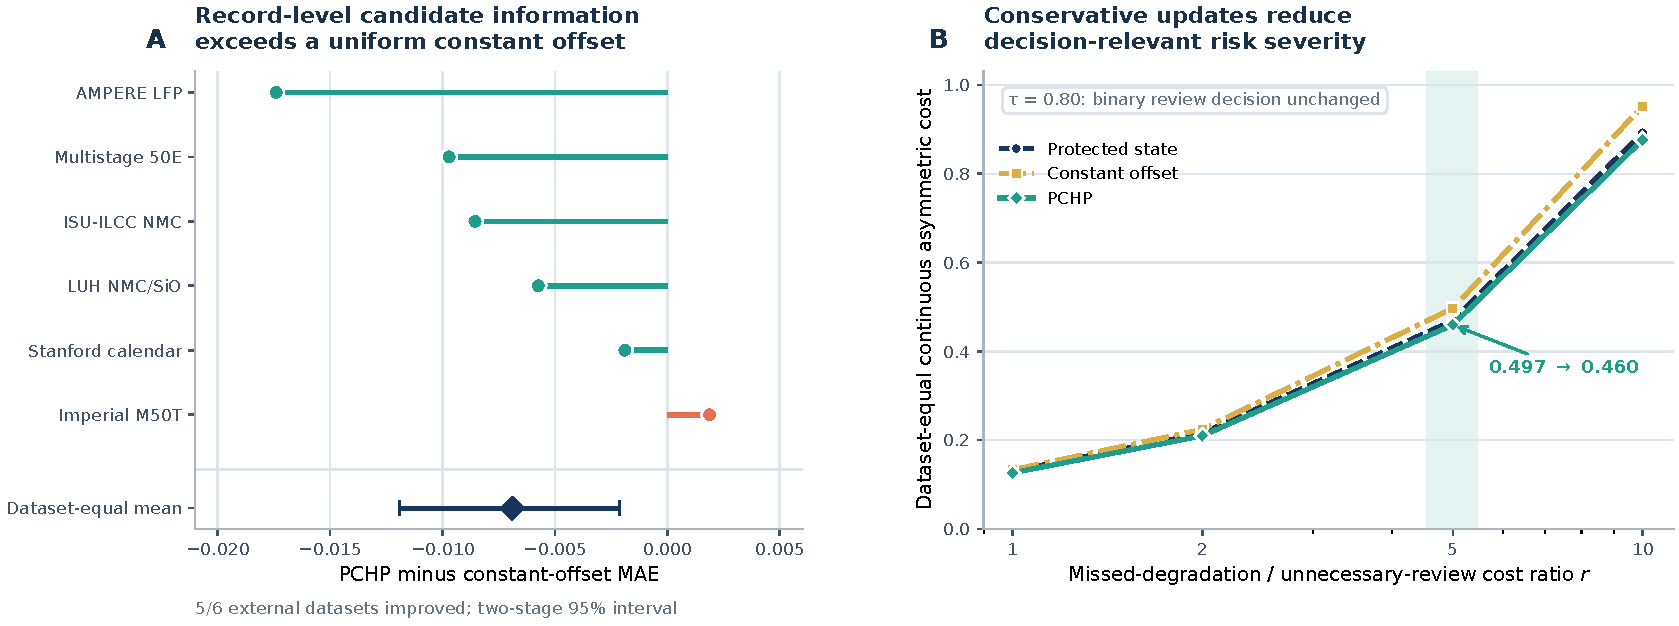
\includegraphics[width=\textwidth]{fig7_external_mechanism_decision.pdf}
  \caption{Protocol-frozen external mechanism confirmation and decision-cost analysis. \textbf{A}, PCHP-minus-development-selected-constant-offset MAE on six external battery datasets; negative values favor PCHP, and the diamond with interval reports the dataset-equal mean and two-stage dataset--cell bootstrap $95\%$ interval. \textbf{B}, dataset-equal continuous asymmetric cost as the missed-degradation-to-unnecessary-review cost ratio increases. At the primary $r=5$, PCHP lowers cost relative to both the constant offset and protected state. The binary review decision at $\tau=0.80$ remained unchanged. Records are nested within $659$ cells and cells within six datasets.}
  \label{fig:external_mechanism_decision}
\end{figure}

\subsection{A strong unprotected comparator exposes the harm-control--accuracy trade-off}

The source-tuned unprotected causal comparator reduced domain-equal MAE from $0.07524$ to $0.05470$. Its paired difference from the protected baseline was $-0.02054$ with a $95\%$ domain-bootstrap interval of $[-0.03364,-0.00675]$ and wins/ties/losses of $10/0/2$. PCHP retained $23.7\%$ of this gain: its MAE exceeded the unprotected comparator by $0.01568$, with interval $[0.00350,0.02725]$ and wins/ties/losses of $3/0/9$. After merging MICH and MICH\_EXP, utility retention was $24.9\%$ and the same qualitative conclusion held.

This additional accuracy was not matched for harm control. The unprotected comparator exceeded the $\delta=0.01$ displacement budget in $524{,}165$ of the $601{,}932$ scored records ($87.08\%$); every one of the $12$ domains and $586$ cells contained at least one violation, and the maximum displacement was $0.35680$. The two record counts therefore refer to the complete scoring roster and its violating subset, respectively. PCHP had no budget violation. The comparison rules out an accuracy-dominance claim: PCHP does not beat the strongest causal candidate on accuracy. Its contribution is to remain inside a declared worst-case harm region while retaining a measurable fraction of the available utility.

\subsection{BaSyTec validation under the prespecified deployment constraints}

The BaSyTec evaluation met all prespecified criteria. Of the $47$ evaluation cells, $45$ satisfied the frozen reference-capacity range, yielding $2{,}969$ scored cycles. Cell-equal MAE changed from $0.17496$ for the protected causal baseline to $0.16510$ for PCHP. The paired difference was $-0.00986$; its paired-cell bootstrap $95\%$ interval extended from $-0.01000$ to $-0.00959$, and all $45$ eligible cells improved. Independent reconstruction matched every cell aggregate within $10^{-12}$. A post-hoc condition-equal sensitivity was negative in all $23$ represented temperature--C-rate conditions, with an interval from $-0.01000$ to $-0.00958$. Maximum PCHP displacement and maximum observed absolute-loss regret were $0.01$ within floating-point tolerance, while the maximum cell-level MAE difference was $-0.00465$.

Both cells at $0\,^{\circ}\mathrm{C}$ and $1.5C$ were excluded by the prespecified $0.08\,\mathrm{Ah}$ lower reference bound: F0009 and F0048 had first-five medians of $0.06862$ and $0.06935\,\mathrm{Ah}$. A clearly post-hoc sensitivity that included them preserved the result across all $47$ cells and all $24$ conditions: the paired difference was $-0.00986$, its interval was $[-0.01000,-0.00961]$, and $47/47$ cells improved. This sensitivity shows that the exclusion did not create the effect, but it does not replace the frozen $45$-cell estimand.

The same evaluation exposes why the empirical claim must remain narrow. The source-tuned unprotected comparator attained MAE $0.06172$, but its maximum displacement was $0.28508$ and it violated the budget in every eligible cell and all $2{,}969$ records; PCHP retained only $8.7\%$ of its accuracy gain. Moreover, the protected baseline underpredicted every scored record, PCHP saturated the positive $0.01$ boundary in $99.1\%$ of records, and a post-hoc fixed $+0.01$ offset achieved MAE $0.16496$, marginally below PCHP by $0.00014$. Thus, Figure~\ref{fig:basytec} evaluates the frozen harm-and-utility constraint and quantifies its accuracy trade-off; this external dataset alone does not distinguish adaptive PCHP behavior from a simple budget-feasible bias correction.

\begin{figure}[t]
  \centering
  
\includegraphics[width=\textwidth]{fig6_basytec_confirmation.pdf}
  \caption{Outcome-blind, protocol-locked BaSyTec external validation and harm-control--accuracy trade-off. \textbf{A}, paired PCHP-minus-baseline MAE for all $45$ eligible cells; negative values favor PCHP. The diamond and interval are the cell-equal mean and $95\%$ paired-cell bootstrap interval from $100{,}000$ resamples. \textbf{B}, cell-equal MAE against maximum pointwise displacement from the protected baseline. PCHP remains inside the declared $\delta=0.01$ region. The fixed $+0.01$ offset is a post-hoc diagnostic, whereas the source-tuned unprotected comparator is prefix causal but violates all eligible-cell budgets. Cycles are nested within cells.}
  \label{fig:basytec}
\end{figure}

\begin{table}[H]
\centering
\caption{Key paired effects. Differences are compared-method minus reference MAE; intervals resample the stated independent unit, not individual records. The unprotected row shows the attainable accuracy gain without the harm-budget constraint.}
\label{tab:primary}
\small
\resizebox{\textwidth}{!}{%
\begin{tabular}{lrrrrl}
\toprule
Evidence tier and comparison & Independent unit & Reference MAE & Compared MAE & Difference & $95\%$ interval \\
\midrule
Nested development & 12 domains & 0.07524 & 0.07038 & $-0.00486$ & $[-0.00671,-0.00301]$ \\
PCHP vs matched constant offset & 12 domains & 0.07515 & 0.07038 & $-0.00477$ & $[-0.00808,-0.00159]$ \\
External confirmation: PCHP vs constant offset & 6 datasets & 0.13326 & 0.12636 & $-0.00690$ & $[-0.01192,-0.00212]$ \\
External confirmation: PCHP vs protected state & 6 datasets & 0.13061 & 0.12636 & $-0.00424$ & $[-0.00745,-0.00079]$ \\
Unprotected candidate vs baseline & 12 domains & 0.07524 & 0.05470 & $-0.02054$ & $[-0.03364,-0.00675]$ \\
BaSyTec PCHP vs baseline & 45 cells & 0.17496 & 0.16510 & $-0.00986$ & $[-0.01000,-0.00959]$ \\
\bottomrule
\end{tabular}%
}
\end{table}

\section{Discussion}

\subsection{What capability changes}

PCHP changes the operational contract of cross-domain battery prediction. A learned model remains responsible for proposing a useful update, but it no longer has unilateral authority over a deployed record. The protected causal state defines the prediction to be preserved, and Corollary~\ref{cor:viability_kernel} identifies the recursive feasible interval as the exact set of current outputs that remain extendable under every future non-increasing protected-state path. Corollary~\ref{cor:optimality} then shows that the final output is not an arbitrary point in that kernel: it is the unique update that preserves maximum fidelity to the current learned proposal under the complete declared constraint set. Theorem~\ref{thm:nonexpansive} adds that the complete recursive cascade cannot magnify a bounded discrepancy in either frozen predictor when the output contract is fixed. The resulting guarantees are simultaneously outcome agnostic and executable online. This is different from retrospective smoothing, which may be label free yet still violates the future-information boundary, and from unconstrained target adaptation, whose gain can become negative in an unknown domain.

The secondary-backbone analysis adds an empirical boundary to that structural claim: the same frozen output constraints remained useful for one linear and two boosting families without backbone-specific retuning. It rules out ExtraTrees-specific utility within the evaluated families, not dependence on every possible candidate architecture.

Theorem~\ref{thm:harm_region} also prevents a misleading interpretation of ``safe'' updating. Without assumptions on the hidden outcome, no method can move a point prediction and remain no worse than its baseline for every possible truth. A positive budget is therefore not a proof relaxation introduced for convenience; it is the unavoidable price of allowing any nontrivial outcome-free update. PCHP makes that price explicit and then spends it only inside the exact intersection with the online trajectory constraints.

The matched controls establish that PCHP is more than conservative clipping. On development domains, record-level changes from the commissioning reference remained useful after both the budget-feasible constant offset and assimilation rate were matched, and the advantage persisted throughout the positive budget grid. The protocol-frozen experiment then reproduced this separation on six external datasets: PCHP won on five datasets and reduced dataset-equal error by $5.18\%$ relative to the exact development-selected offset. This is direct external evidence for the algorithmic mechanism: adaptive candidate information contributes value within a fixed output constraint. It does not identify a microscopic electrochemical pathway, which was not the mechanism claim being tested.

\subsection{Battery-specific operational meaning}

The projection theory can be reused outside batteries, but the present constraint is driven by a battery-specific decision problem. In a swapping station, fleet depot, or warranty-monitoring program, partial charge measurements arrive during routine service while reference capacity requires a deliberately scheduled characterization \citep{liu2023rapid,zhang2024flexible}. A supplier, chemistry, or protocol shift can invalidate the source calibration precisely when an operator must decide whether to continue service or request a diagnostic. PCHP uses charge-response changes from the commissioning reference to adapt the estimate immediately, limits how much the unverified update can worsen the protected prediction, and prevents later measurements from rewriting the decision history. The external decision-cost analysis shows the practical consequence: under a $5{:}1$ missed-degradation-to-unnecessary-review cost ratio, decision-relevant error severity fell by $7.54\%$ relative to the matched constant offset, while the binary review decision at $80\%$ retention remained unchanged. Long-term capacity fade motivates the non-increasing emitted trend; raw observations should remain available to diagnose short-term recovery or measurement rebound.

\subsection{Meaning of the BaSyTec evaluation and the harm-control--accuracy trade-off}

The BaSyTec experiment tests whether a prediction artifact frozen before capacity access improves its protected baseline while preserving all declared harm checks under a new laboratory, cell type, and $24$-condition stress grid. It passes that test, and the post-hoc full-condition sensitivity shows that the prespecified low-reference exclusion did not generate the direction of effect. Because the scored cells remain within the prespecified model-support range, the result supports relative utility under the declared target contract. It does not convert their condition-specific aging-cycle capacities into standardized RPT SOH or establish electrochemical validity outside the tested protocols.

BaSyTec exhibits an almost uniform baseline underprediction, so a fixed positive offset performs marginally better there. That result remains valuable: it shows that the frozen deployment constraint transfers to a new laboratory program and quantifies the accuracy forgone by enforcing the harm budget. The six-dataset confirmation answers the complementary question that BaSyTec alone could not answer; under heterogeneous error directions, PCHP outperformed the development-selected constant offset while satisfying every deterministic check. Together, the experiments separate constraint transfer from adaptive-mechanism value instead of asking one dataset to prove both.

\subsection{Choosing the harm budget}

The budget $\delta$ is expressed in normalized-capacity units and controls a transparent engineering trade-off: a smaller value protects the inherited record more tightly, whereas a larger value admits more adaptive gain. The frozen $\delta=0.01$ limited every external update to one normalized-capacity percentage point and, in the six-dataset audit, reduced continuous decision cost without changing the binary review decision at $80\%$ retention. This operating point is conservative and practically interpretable; a different fleet can select a different point from its maintenance and warranty consequences. The supplementary theory appendix gives the exact directional radii for unequal consequences and the minimum time-varying budget compatible with an already issued prefix.

For engineering calibration, first fix the protected decision, asset horizon, and cost boundary---for example maintenance timing, avoidable downtime, warranty exposure, or a separately justified safety-related consequence. For a prediction $p$ and later measured retention $y$, use the local directional approximation
\begin{equation}
  \ell_{\mathrm{eng}}(p,y)
  =c_{\mathrm{under}}(y-p)_{+}
  +c_{\mathrm{over}}(p-y)_{+},
  \label{eq:engineering_cost}
\end{equation}
where $p<y$ represents retention underestimation and potentially premature intervention, whereas $p>y$ represents retention overestimation and potentially delayed intervention. The weights should be estimated from operator records or a preregistered engineering elicitation over a small declared perturbation $\Delta y>0$,
\begin{equation}
  c_{\mathrm{under}}=\frac{\Delta C_{\mathrm{early}}}{\Delta y},
  \qquad
  c_{\mathrm{over}}=\frac{\Delta C_{\mathrm{late}}}{\Delta y}.
  \label{eq:engineering_weights}
\end{equation}
The exercise should replay both signed perturbations through the same maintenance or warranty rule, stratify weights when chemistry, duty cycle, or asset age materially changes cost, and freeze the selected point estimate or conservative quantile before evaluating target outcomes. A decision-loss budget $\eta$ then gives the standalone admissible interval
\begin{equation}
  \left[b-\frac{\eta}{c_{\mathrm{under}}},
        b+\frac{\eta}{c_{\mathrm{over}}}\right].
  \label{eq:engineering_interval}
\end{equation}
For the present audit, normalized weights provide a reproducible consequence ratio and yield the observed $7.54\%$ reduction at $r=5$. Deployment owners can replace them with monetary, downtime, warranty, or validated safety weights from their own ledgers. If the true rule is strongly nonlinear, the corresponding decision loss should replace Eq.~\eqref{eq:engineering_cost} and its feasible set should be re-derived.

\subsection{Statistical interpretation}

The deterministic certificate is pointwise and requires no sampling assumption. Empirical utility uncertainty follows the data hierarchy. Twelve complete domains support the development effect; $601{,}932$ records are repeated observations, not independent transfers. In the external mechanism confirmation, six datasets are the top-level transport units and $659$ cells are nested replicates, so the bootstrap resamples datasets and then cells. BaSyTec uses $45$ cells for its frozen within-program effect. The intervals therefore quantify heterogeneity at the level relevant to each claim without inflating evidence through pooled records.

The finite-sample sensitivity preserved the negative mean direction without relying on the percentile bootstrap alone. For the primary effect and the integrated budget path, exact sign-flip values were $0.00098$ and $0.00781$, and Student-$t$ $95\%$ intervals were $[-0.00703,-0.00269]$ and $[-0.01172,-0.00217]$, respectively. For PCHP versus the matched constant-offset control, the corresponding values were $0.01660$ and $[-0.00858,-0.00097]$. However, its direction-only sign-test value was $0.145996$ because PCHP won in $9/12$ domains. The supported claim is therefore a domain-equal mean utility contribution with heterogeneous domain effects, not universal dominance or a claim that a randomly drawn new domain is more likely than not to improve. All values are descriptive post-hoc sensitivities on opened development domains.

Confirmation strength follows from whether the evaluation evidence influenced the tested design. BaSyTec is outcome blind because its predictions were fixed before capacity access. The six-dataset experiment uses a different but legitimate boundary: the archives had historical exposure in unrelated branches, yet none of their outcomes or summaries changed PCHP, the comparator, estimand, cost protocol, or decision criteria before the frozen run. It therefore provides protocol-frozen external mechanism confirmation on datasets that did not influence the tested design. These two designs offer complementary evidence, while future independent laboratory replication can extend the transport scope further.

\section{Limitations and failure modes}

The guarantee is relative to the specified protected causal state. PCHP controls the incremental harm of an update; it does not repair a biased baseline, incompatible capacity label, distribution shift, or unsafe battery. Likewise, nonexpansiveness controls algorithmic perturbation propagation rather than calibration or physical risk. The metric-loss theorem and bounded squared-loss construction require their stated outcome spaces, and a new discontinuous decision loss requires its own feasible-set derivation.

Strict non-increase is an operational trend representation and can suppress genuine short-term capacity recovery or measurement rebound, so raw observations and projected trends should both be retained. The first-five commissioning anchor can also fail when a cell enters monitoring after unobserved aging or when its initial records are corrupted. PCHP currently returns a bounded estimate rather than abstaining; a future estimability gate would be a useful complementary component.

The empirical scope is broad but based on public data. The twelve-domain analyses are retrospective development evidence. The six external datasets had historical exposure in unrelated branches, although their outcomes did not affect the frozen method or evaluation protocol. BaSyTec is outcome blind but represents one laboratory program; its two low-reference cells were excluded by the frozen support rule. The supplementary NASA analysis is retained only as a one-program stress test of an incompatible absolute target, not as utility evidence for absolute capacity-retention estimation \citep{saha2007nasa}. These boundaries motivate prospective fleet replay and independent laboratory replication across additional chemistries and duty cycles. Finally, the normalized decision-cost ratios show operational relevance but do not replace site-specific monetary, downtime, warranty, or safety-cost calibration.

\section{Conclusion}

PCHP makes learned cross-domain battery-health updates executable before capacity outcomes arrive. It converts the protected prediction into a prefix-causal state and admits a candidate based on changes from the commissioning reference only through the exact recursively feasible harm-budget interval. This construction provides prefix invariance, non-increasing output, $O(1)$ online execution, a tight pointwise absolute-loss bound, and prefix-wise $\ell_\infty$ nonexpansiveness. Across twelve development domains, PCHP reduced domain-equal MAE by $0.00486$ while every update respected the $0.01$ budget. The protocol-frozen confirmation on six external datasets then showed that the adaptive candidate outperformed the exact development-selected constant budget-feasible offset by $0.00690$ across $659$ cells, with a two-stage $95\%$ interval entirely below zero. At a $5{:}1$ missed-degradation cost ratio, continuous decision risk fell by $7.54\%$ without changing the binary review decision at $80\%$ retention. BaSyTec confirmed transfer of the deployment constraint under a new laboratory program, while the unprotected comparator quantified the accuracy trade-off created by enforcing the harm budget. These results establish PCHP as a rigorous and practical risk-control layer for adaptive lithium-ion battery capacity-retention estimation.

\section*{Declaration of generative AI and AI-assisted technologies in the manuscript preparation process}

During the preparation of this work, the first author used OpenAI Codex to assist with research-code development and verification, literature-search organization, manuscript structuring, translation, and language editing. The first author manually reviewed and independently verified the source claims, mathematical derivations, analyses, code outputs, figures, and text. The authors retain responsibility for the final manuscript. All scientific figures were generated programmatically from the reported data and scripts; no generative image model was used to create or alter manuscript figures.

\section*{CRediT authorship contribution statement}

Yuyang Wu: Conceptualization, Methodology, Software, Validation, Formal analysis, Investigation, Data curation, Visualization, Writing -- original draft, Writing -- review and editing. Aiping Jiang: Supervision, Project administration, Writing -- review and editing.

\section*{Data availability}

The exact development snapshot, BatteryLife\_Processed v11, is archived on Zenodo under CC BY~4.0 \citep{batterylife2026processed}. The six-dataset confirmation uses the cited A123/LFP, Imperial M50T 21700, Luh NMC/C--SiO, ILCC varying-usage, Stanford calendar-aging, and multistage-aging sources \citep{wheeler2025lfp,kirkaldy2024comprehensive,luh2024dataset,li2024varyingusage,lam2025calendar,stroebl2024multistage}. The $48$-cell Bayreuth degradation-path dataset is available from Zenodo under CC BY~4.0 \citep{roder2025degradationdata}. Every third-party archive remains governed by its provider's access, attribution, and redistribution terms and is not redistributed here. The author-created reproducibility release contains acquisition instructions, source and artifact hashes, frozen external protocols, aggregate dataset- and cell-level evidence, independent certificate and statistical replay checks, and all figure-generation inputs and scripts. It is publicly available under the MIT License in the \href{https://github.com/xiansuqiushui-dotcom/pchp-battery-capacity-retention}{public GitHub repository}. This release does not supersede any third-party terms; complete refitting and external replay require provider-authorized downloads.

\section*{Funding}

This research received no specific grant from any funding agency in the public, commercial, or not-for-profit sectors.

\section*{Declaration of competing interest}

The authors declare that they have no known competing financial interests or personal relationships that could have appeared to influence the work reported in this paper.

\begingroup
\hbadness=2000
\bibliographystyle{elsarticle-num}
\bibliography{references}
\endgroup

\end{document}
